
\ifdraft{\color{green}}{}\chapter{Desenvolvimento da Aplicação}

A criação do protótipo desse sistema foi o ponto principal desse trabalho, pois os objetivo foi oferecer opção para substituir \textit{softwares} que vêm sendo utilizados atualmente por um prático, atual, acessível e com o código disponível para que possa ser corrigido e melhorado. Essencialmente a aplicação foi desenvolvida em linguagens Web, o JavaScript sendo a linguagem de programação, HTML como linguagem de marcação e CSS como estilização.

Nesse protótipo buscou-se eliminar algumas deficiências básica que existem em ferramentas similares, por exemplo funcionalidade de desfazer durante a edição, pois essas podem fazer com que o seu uso seja desgastante e desanimador. Como mencionado nas limitações a inclusão de funcionalidades que poderiam estar disponíveis ficarão como sugestões, algumas delas são encontradas por exemplo em Ambientes Integrados de Programação, comumente utilizada em outras linguagens.

\begin{figure}[h]
  \ifdraft{\color{green}}{}\caption{\ifdraft{\color{green}}{}Interpretador proposto}\label{fig:analisador}
  \centering

\includegraphics[width=\textwidth,height=10cm,keepaspectratio]{figures/interpretador-proposto.pdf}
  \caption*{\ifdraft{\color{green}}{}\footnotesize Fonte: Produção do autor, baseado em \citeonline{esmin1998}.}
\end{figure}

Inclusive há caso em que a ferramenta inicialmente utilizada não é capaz de executar alguns algoritmos mais avançados. E isto leva a necessidade do uso de outro software na mesma disciplina até com possivelmente uma nova linguagem (por exemplo a linguagem de programação C ou C++), devido a está necessidade alguns educadores optam por esta sendo a única ferramenta utilizada, ignorando linguagem Portugol. Espera-se que diferente o UAL essa limitação possa realmente ser concluída em trabalho futuros, conforme proposto nas conclusões.

\section{Levantamento de Requisitos}

% NOTE Seguindo o modelo de \citeonline{silva2013} de um AVA

O desenvolvimento de \textit{software} antes de iniciar a códificação algumas esta[as são esperadas e recomendadas para maior acertividade (qualidade, orçamento, prazos). Análise requisitos prioriza e classifica os pontos aos quais a aplicação se pretende solucionar.

\subsection{Requisitos Funcionais}

\begin{enumerate}

\item Permitir ao aluno edição de código

\item Permitir ao aluno abrir arquivos de texto

\item Permitir salvar o arquivo alterado

\item Permitir visualizar a simulação do programa

\end{enumerate}

\subsection{Requisitos Não Funcionais}

\begin{enumerate}

\item O programa deve prezar pelo menor tamanho possível nos arquivos

\item O sistema deverá rodar em navegador (\textit{browser}) moderno

\item Deverá ter interface minimalista, mas visualmente agradável

\item Permitir visualizar a simulação do programa

\end{enumerate}

\begin{figure}[h]
  \caption{\ifdraft{\color{green}}{}Caso de uso Aluno}\label{fig:usecase}
  \centering
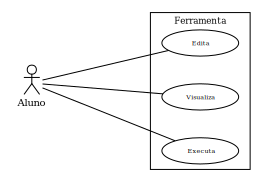
\includegraphics[width=.8\textwidth,height=10cm,keepaspectratio]{figures/caso-de-uso.pdf}
  \caption*{\ifdraft{\color{green}}{}\footnotesize Fonte: Produção do autor.}
\end{figure}

\section{Editor de Código ACE}

No modelo para navegador já existem editores de código fonte de linguagens de programação,dos mais utilizados temos ACE\nocite{ace} e o CodeMirror\nocite{codemirror}, optado pelo primeiro pois em análise entendeu-se como sendo mais prático para o uso e criação do modelo da linguagem. Considerou-se a criação do modelo gramatical para destaque da sintaxe como dificuldade relativamente baixa.

Em tecnologia há os chamados \textit{playground} (área de lazer), que são chamadas áreas para experimentações com determinada ferramenta ou tecnologia. No caso do editor ACE é disponibilizado uma ``pia de cozinha'' (\textit{Kitchen Sink}\nocite{kitchensink}) conforme figura \ref{fig:ace-kitchensink}, onde o editor embutido pode ser modificado através de um menu lateral quanto a linguagem ou tema e outras de suas várias opções.

\begin{figure}[h]
  \caption{\ifdraft{\color{green}}{}Ace \textit{Kitchen Sink}}\label{fig:ace-kitchensink}
  \centering
\includegraphics[width=\textwidth,keepaspectratio]{figures/ace-kitchensink.pdf}
  \caption*{\ifdraft{\color{green}}{}\footnotesize Fonte: Captura de tela da parte visível no navegador.}
\end{figure}

Inicialmente as funcionalidades pretendidas são todas supridas e outra mais levam a esta ser uma opção útil para evolução da aplicação em trabalhos futuros. Ignorando as duas que dizem respeito ao destacamento de sintaxe em mais de 110 linguagens (porem custumizável, que permitiu adicionar UAL) e mais de 20 temas (também personalizado apra o preto com negrito nas palavras reservadas, como o Editor UAL), as outras seguem listadas:

\begin{itemize}

\item Identação automática;
\item Permite documentos com muitas linhas;
\item Atalhos de teclado personalizáveis;
\item Localizar e substituir, podendo utilizar expressões regulares;
\item Alternar entre tabulação suave (espaços) ou tabulação real;
\item Exibir caracteres ocultos;
\item Arrastar e soltar utilizando mouse;
\item Limitação de colunas no texto, com quebra;
\item Retrair ou expantir código/
\item Cursores e seleção múltiplas;
\item Checagem em tempo real para algumas linguagens/
\item Funcionalidade de recortar, copiar e colar.

\end{itemize}

\section{Acorn}

Para resultar na árvore sintática encontrou-se o ACORN\nocite{acorn} um parser já escrito em JavaScript. De modo trabalhoso foi necessário adaptar o código fonte para compreender a estrutura do algorítmos proposto, principalmente devido à não utilização de parênteses para o comando de impressão em tela na linguagem UAL.

\begin{quadro}[h]
\centering
  \caption{Árvore sintática gerada pelo Acorn modificado}\label{qua:compare-tools}
\begin{lstlisting}[style=json,frame=single]
{
  "type": "Program",
  "start": 0,
  "end": 61,
  "body": [
    {
      "type": "PrintStatement",
      "start": 19,
      "end": 53,
      "print": {
        "type": "CallPrint",
        "start": 27,
        "end": 52,
        "arguments": {
          "type": "Literal",
          "start": 27,
          "end": 52,
          "value": "Aprendendo Algoritmo!!!",
          "raw": "\"Aprendendo Algoritmo!!!\""
        }
      }
    }
  ],
  "id": {
    "type": "Identifier",
    "start": 5,
    "end": 16,
    "name": "algoritmo11"
  }
}
\end{lstlisting}
  \caption*{\ifdraft{\color{green}}{}\footnotesize Fonte: Produção do autor.}
\end{quadro}

\section{JS-Interpreter}

Como saída o interpretada o JS-Interpreter\nocite{jsinterpreter} foi encontrado como a única opção. Ele já se utiliza do mesmo ACORN mencionado acima e interpreta a própria linguagem JavaScript. Pelo mesmo motivo citado acima, falta de parênteses no comando, se tornou uma tarefa um tanto dispendiosa fazer com que ele se adaptasse ao modelo.

\begin{figure}[h]
  \caption{Esquemático do Interpretador}\label{fig:flux}
  \centering
  \setlength{\fboxsep}{0pt}%
\setlength{\fboxrule}{1pt}%
\fbox{
\includegraphics[width=10cm,height=10cm,keepaspectratio]{figures/bizual-interpretador.pdf}}
  \caption*{\footnotesize Fonte: Produção do autor.}
\end{figure}

\section{Interface Gráfica}

Como interface gráfica foi mantido o mínimo necessário. Somente o editor de texto e um botão para executar. Foram visualizadas renderizações e tamanhos de telas variados, computadores (Figura \ref{fig:ui-pc}), tablets, smartphones (Figura \ref{fig:ui-phone}), etc. Seguindo conceitos do Google Material Design foi adicionada uma barra no topo como botão para menu o nome da aplicação, denominada Bizu, e um botão flutuante no canto inferior direito como ícone ``play'' para a execução do algoritmo.

\begin{figure}[h]
  \caption{Interface Desktop}\label{fig:ui-pc}
  \centering
  \setlength{\fboxsep}{0pt}%
\setlength{\fboxrule}{1pt}%
\fbox{\includegraphics[width=10cm,height=10cm,keepaspectratio]{figures/bizual-desktop.pdf}}
  \caption*{\footnotesize Fonte: Produção do autor.}
\end{figure}

De acordo com o \citeonline{dicionarioinformal2016} a gíria ``bizu'' teve origem em quartéis militares, onde os experientes sussurravam dicas para os novatos. Os superiores de longe ouviam aquela onomatopéia característica de cochicho ``bzbzbzu'', dando origem ao termo. A escolha do nome se deve a partir da palavra bizu adicionada a sigla da sintaxe: resultando em ``BizUAL'', nesta grafia.

\begin{figure}[h]
  \caption{Interface Smartphone}\label{fig:ui-phone}
  \centering
  \setlength{\fboxsep}{0pt}%
\setlength{\fboxrule}{1pt}%
\fbox{\includegraphics[width=10cm,height=10cm,keepaspectratio]{figures/bizual-smartphone.pdf}}
  \caption*{\footnotesize Fonte: Produção do autor.}
\end{figure}

Facilitando a tarefa de construção da interface foi utilizada a biblioteca Material Design Lite (MDL)\nocite{mdl} disponibilizada oficialmente pelo Google. As cores foram escolhidas pela funcionalidade disponível no site da biblioteca.

Foi utilizado a funcionalidade \textit{app cache} a partir de um arquivo manifesto listando o conteúdo que o navegador deve guardar cópia local. Podendo assim ter a internet desconectada após o primeiro acesso que a aplicação continuará acessível.

Todo o código foi desenvolvido em repositório disponível no github e quando concluído em sua versão mínima movido para seu destino final e podendo ser acessado.\nocite{bizual}\color{black}

\section{\textit{AppCache}}

Desenvolvido pela consórcio criado para o desenvolvimento do HTML5 veio suprir a necessidade de armazenamento avançado de arquivos utilizados na aplicação web. Utiliza apenas um arquivo de texto onde lista todos os arquivos de imagem, estilização, scripts de programação, entre outros (ver quadro \ref{qua:html-root}). Esse arquivo declarado manifesto deve ser desclarado como atributo no etiqueta de abertura do html (veja quadro  \ref{qua:cache-appcache}).

\let\origthelstnumber\thelstnumber
\makeatletter
\newcommand*\Suppressnumber{%
  \lst@AddToHook{OnNewLine}{%
    \let\thelstnumber\relax%
     \advance\c@lstnumber-\@ne\relax%
    }%
}

\newcommand*\Reactivatenumber[1]{%
  \lst@AddToHook{OnNewLine}{%
   \let\thelstnumber\origthelstnumber%
   \setcounter{lstnumber}{\numexpr#1-1\relax}%
   %\advance\c@lstnumber\@ne\relax%
  }%
}

\makeatother

\begin{quadro}[h]
\centering
  \caption{Código HTML ignorando cabeçalho e corpo}\label{qua:html-root}
\begin{lstlisting}[numbers=left,escapeinside=\$\$,frame=single]
<!DOCTYPE html>
<html lang="pt-BR" manifest="cache.appcache">
  <head>$\Suppressnumber$
    (...)$\Reactivatenumber{16}$
  </head>$\Reactivatenumber{17}$
  <body>$\Suppressnumber$
    (...)
  </body>$\Reactivatenumber{51}$
</html>

\end{lstlisting}
  \caption*{\ifdraft{\color{green}}{}\footnotesize Fonte: Produção do autor.}
\end{quadro}

\begin{quadro}[h]
\centering
  \caption{Arquivo de manifesto \textit{appcache}}\label{qua:cache-appcache}
\begin{lstlisting}[numbers=left,frame=single]
CACHE MANIFEST

# Adds the ability to play the game offline.
# The following comment needs to be updated whenever a change is made.
# Run `rake appcache:update` to do so
# Updated: 2016-11-90T01:27:00-02:00

# Main page

# CSS
style/material.blue-orange.min.css
style/main.css

# Fonts
style/fonts/material-icons.css
style/fonts/MaterialIcons-Regular.eot
style/fonts/MaterialIcons-Regular.woff
style/fonts/MaterialIcons-Regular.woff2
style/fonts/MaterialIcons-Regular.ttf

# Other resources

# JavaScript
js/material.min.js
js/aceual.js

favicon.ico

NETWORK:
*

\end{lstlisting}
  \caption*{\ifdraft{\color{green}}{}\footnotesize Fonte: Produção do autor.}
\end{quadro}

\ifdraft{}{
%\section{Ferramentas Utilizadas}

%
%
%\section{Processo Criacional}
%
%\subsection{Git e Github}
%
%\subsection{Node.js e Grunt}
%
%\subsection{SASS}
%
%\subsection{TDD}
%
%\subsection{\textit{Material Design}}
%
%\subsubsection{MDL}
%
%\subsection{Inspirações}
}
